\documentclass{beamer}
\mode<presentation>
{
\usetheme{Madrid}
\usecolortheme{seagull}
}

\usepackage{graphicx}
\usepackage{amsmath}
\usepackage{amssymb}

\title[AWS Workshop]{AWS Workshop} 

\author{Jaime Canizales} 
\institute[Hunter College] 
{
City University of New York \\ 
\medskip
\textit{jaime.canizales@hunter.cuny.edu} 
}
\date{\today} 
\begin{document}


\begin{frame}
\titlepage 
\end{frame}


\begin{frame} \frametitle{Overview} 
\tableofcontents
\end{frame}


\section{Introduction}
\begin{frame}\frametitle{What is AWS?}
\begin{block}{Problem Statement}
AWS (Amazon Web Services) is a comprehensive cloud computing platform 
provided by Amazon. It offers a wide range of on-demand services, such as 
compute power, storage, databases, and networking, as well as advanced 
technologies like machine learning, artificial intelligence, Internet of Things (IoT),
and more. AWS enables individuals, businesses, and organizations to build and deploy 
applications without the need to own or manage physical hardware.
\end{block}
\end{frame}


\begin{frame}\frametitle{Why use AWS? Part 1}
\begin{itemize}
\item AWS provides a great solution to scaling. As our software grows in demand, 
the servers hardware must also scale to match it. This can be expensive because
more hardware cost most more money, physical space, set up hassels and so forth. 
AWS provides servers across the the world, that remove the hassel of owning 
your own local servers, and provide computational speed ups as you can have 
servers all over the world in the case your software goes international.    
\end{itemize}
\end{frame}


\begin{frame}\frametitle{Why use AWS? Part 2}
\begin{itemize}
\item AWS solves the crossplatform development issue. In aws you can standardize
the development of your software so that all your engineers can test and 
deploy on the same cloud network and computers!   
\end{itemize}
\end{frame}


\begin{frame}\frametitle{Why use AWS? Part 3}
\begin{itemize}
\item AWS is the most used of all the cloud computing services. (others: Microsoft azure, google cloud, ...)
\item You are most likely to use this cloud computing service when you get a job
\item One of the easier cloud computing services to learn because there is a lot of documentation due to its extensive use in the industry.    
\end{itemize}
\end{frame}

\begin{frame}{Some key services offered by AWS include:}
\begin{itemize}
\item Amazon EC2 (Elastic Compute Cloud): Virtual servers to run applications.
\item Amazon S3 (Simple Storage Service): Scalable object storage for files and data.
\item Amazon RDS (Relational Database Service): Managed relational databases like MySQL, PostgreSQL, and Oracle.
\item AWS Lambda: Serverless computing to run code without managing servers.
\end{itemize}
\end{frame}


\begin{frame}{More key services:}
\begin{itemize}
\item Amazon CloudFront: Content delivery network (CDN) for delivering websites and applications globally.
\item AWS is known for its scalability, reliability, and cost-effectiveness, serving both startups and large enterprises worldwide.
\item IAM and Organizations: facilitates collaboration, by using policies to give different permissions to different employees
\item Works well with version control like git! you can set yor git server to build and deploy software from aws(continuous integration)
\item Cloudformation allows you to save network and software architecture set ups to templates
\end{itemize} 
\end{frame}



\section{Conclusion}
\begin{frame}\frametitle{Access Key Setup}
\begin{itemize} 
\item To ease communication with S3 and other servers we must set up an access key.
\item Top righthand click on name, then click on security credentials, then click create access key.
\item Make sure to store the secret key somewhere safe as this is the only time you will see it.
\end{itemize}
\end{frame}


\begin{frame}\frametitle{S3 Setup}
\begin{itemize} 
\item Load files into s3 bucket. \href{https://docs.aws.amazon.com//AmazonS3//latest//userguide//creating-bucket.html}{link}
\item From an EC2 instance you can get files from S3 bucket with command: \textbf{aws s3 cp s3://my2awsbucket/file\_absolute\_path .}
\item From an EC2 instance you can upload files to S3 bucket with command:\textbf{aws s3 cp fileName s3://my2awsbucket/}
\end{itemize}
\end{frame}

    
\begin{frame}\frametitle{EC2 Setup}
\begin{itemize} 
\item Go through creating ec2 instance (you can leave everything as default). \href{https://docs.aws.amazon.com/AmazonRDS/latest/UserGuide/CHAP_GettingStarted.CreatingConnecting.PostgreSQL.html}{link}
\item ssh into ec2 instance, and run \textbf{sudo dnf update -y} and \textbf{sudo dnf install postgresql15} to install psql
\item Run \textbf{aws configure} and add your access key 
\item Reference last slide to get data from S3
\end{itemize}
\end{frame}


\begin{frame}\frametitle{RDS Setup}
\begin{itemize}  
\item Create rds (relational database server) using easy create, postgresql, and connect to ec2 instance. \href{https://docs.aws.amazon.com/AmazonRDS/latest/UserGuide/CHAP_GettingStarted.CreatingConnecting.PostgreSQL.html}{link}
\item ssh back into ec2 instance and run \textbf{psql --host=endpoint --port=5432 --dbname=postgres --username=postgres} to access database server
\item Check out file \href{../commands.sql}{commands.sql} to pass data to sql database
\end{itemize}
\end{frame}

\begin{frame}\frametitle{Connect to vscode}
\begin{itemize}
\item Connect vscode Documentation: \href{https://medium.com/@christyjacob4/using-vscode-remotely-on-an-ec2-instance-7822c4032cff}{link}
\item vscode extension Remote ssh
\item Modify ~/.ssh/config to include networking information of ec2 instance
\end{itemize}
\end{frame}


\begin{frame}\frametitle{Software Architecture}
\begin{figure}
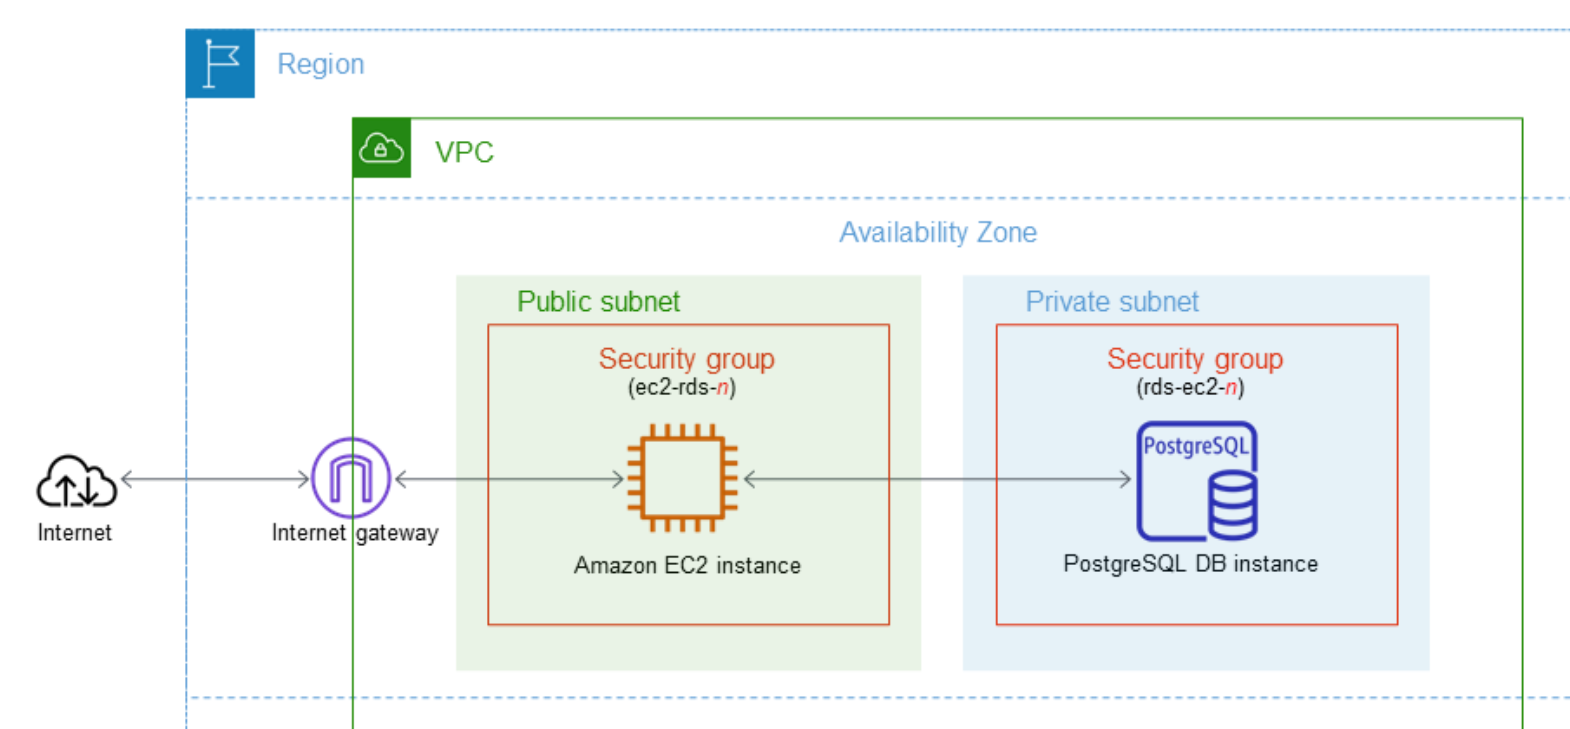
\includegraphics[width=12cm]{software_architecture.png}
\begin{itemize}
\item Ensure everything is in the same vpc(virtual private network), like in picture.
\end{itemize}
\end{figure}  
\end{frame}


\end{document}